\documentclass[tikz,border=2pt]{standalone}
\usepackage{amsmath,amssymb}
\usepackage{tikz}
\usetikzlibrary{arrows.meta,calc}

\begin{document}
% The distance from A to the line l(t) = B + t v is the length of the perpendicular: split
% A - B into its projection onto v and the leftover orthogonal part.
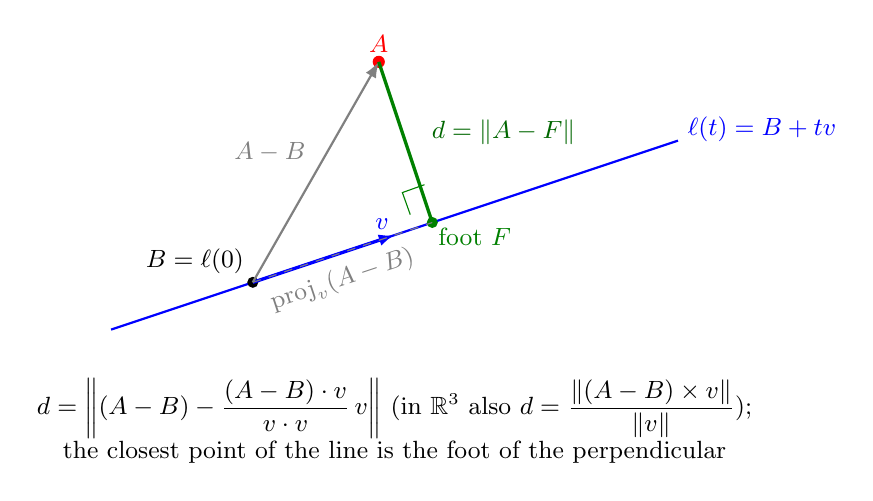
\begin{tikzpicture}[every node/.style={font=\small}, >={Latex[length=2mm]}]
	\draw[blue, thick] (-1.2,-0.4) -- (6.0,2.0);
	\node[blue, anchor=west] at (6.0,2.15) {$\ell(t)=B+tv$};
	\coordinate (B) at (0.6,0.2);
	\coordinate (A) at (2.2,3.0);
	% v = (3,1); foot = B + ((A-B).v/|v|^2) v = (0.6,0.2) + ((1.6*3+2.8*1)/10)(3,1) = (0.6,0.2)+0.76(3,1)
	\coordinate (F) at (2.88,0.96);
	\fill (B) circle (2pt) node[above left, inner sep=3pt] {$B=\ell(0)$};
	\draw[->, blue, very thick] (B) -- (2.4,0.8) node[above left, inner sep=1.5pt, font=\small] {$v$};
	\fill[red] (A) circle (2.2pt) node[above, inner sep=3pt] {$A$};
	\draw[->, gray, thick] (B) -- (A) node[midway, above left, font=\small] {$A-B$};
	\draw[green!50!black, very thick] (A) -- (F);
	\fill[green!50!black] (F) circle (2pt) node[below right, inner sep=2pt, font=\small] {foot $F$};
	\draw[green!50!black] ($(F)+(-0.28,0.1)$) -- ($(F)+(-0.38,0.38)$) -- ($(F)+(-0.1,0.48)$);
	\node[green!40!black, anchor=west, font=\small] at (2.75,2.1) {$d=\|A-F\|$};
	\draw[dashed, gray] (B) -- (F);
	\node[gray, font=\small, rotate=18.43, anchor=north] at (1.65,0.5) {$\operatorname{proj}_v(A-B)$};
	\node[anchor=north, align=center] at (2.4,-0.9) {$d=\left\|(A-B)-\dfrac{(A-B)\cdot v}{v\cdot v}\,v\right\|$ (in $\mathbb{R}^3$ also $d=\dfrac{\|(A-B)\times v\|}{\|v\|}$);\\ the closest point of the line is the foot of the perpendicular};
\end{tikzpicture}
\end{document}
